\documentclass[a4paper]{article}

%% Language and font encodings
\usepackage[english]{babel}
\usepackage[T1]{fontenc}
\usepackage{graphicx}
\usepackage{float}
\graphicspath{ {images/} }

%% Sets page size and margins
\usepackage[a4paper,top=3cm,bottom=2cm,left=3cm,right=3cm,marginparwidth=1.75cm]{geometry}

\usepackage[colorlinks=true, allcolors=blue]{hyperref}

\title{BDSA 2017 Assignment 03}
\author{Martin Winther \and Cæcilie Vildenfeldt Iversen}

\begin{document}
\maketitle

\section{Exercise 1}

\subsection{}
Can the system under consideration be represented as an actor? Justify your answer\\
\\
\textbf{Answer:} No, the system under considereation cannot be represented as an actor when performing requirements elicitation. \\
An actor is an external entity that interacts with the system and therefore the system itself cannot be considered an actor. 
The questions for determining an actor are:
\begin{itemize}
\item Which users are supported by the system to perform work? 
\item Which users execute the main functions? 
\item Which users perform secondary functions (maintenance, operation, etc.)? 
\item With what external system (hw/sw) will the system interact?
\end{itemize}
None of these questions conceivably cover the system itself.

\subsection{}
What is the difference between a scenario and a use case? When do you use each construct?\\
\\
\textbf{Answer:} 
Definitions:
\begin{itemize}
\item \textbf{A scenario} 
\begin{itemize}
\item is an instance of a use case describing a concrete set of actions.
\item is a narrative description of what people do and experience as they try to make use of computer systems and applications.
\item is used as examples for illustrating common cases; their focus is on understandability.
\end{itemize}
\item \textbf{A use case} 
\begin{itemize}
\item is an abstraction that describes all possible scenarios involving the described functionality.
\item represents a complete flow of events through the system in the sense that it describes a series of related interactions that result from its initiation.
\item describes the behavior of the system as seen from an actor’s point of view.
\item is used to describe all possible cases; their focus is on completeness. 
\end{itemize}
\end{itemize}
The difference between a scenario and use case is one of perspective. \\
A scenario is a very narrow description of a set of interactions with the system, while the use case describes the flow of events initiated by an actor in detail.\\
A scenario is used for communicating with the client, they are understandable and do not use much technical language.\\
A use case is used for development and is based upon the requirements set forth by the scenario. It is created as a collaborative effort by the client and developer.


\subsection{}
What is the difference between a state machine diagram and an activity diagram?\\
\\
\textbf{Answer:} 
\begin{itemize}
\item \textbf{A state machine diagram}
\begin{itemize}
\item is a notation for describing the sequence of states an object goes through in response to external events.
\item describes the dynamic behavior of an individual object as a number of states and transitions between these states.
\item focuses on the transitions between states as a result of external events for an individual object.
\end{itemize}
\item \textbf{An activity diagram}
\begin{itemize}
\item describes the behavior of a system in terms of activities.
\begin{itemize}
\item Activities are modeling elements that represent the execution of a set of operations. 
\end{itemize}
\item can be used to represent control flow and data flow.
\item model the dynamic behaviour of a system - show decisions.
\end{itemize}
\end{itemize}
The difference between a state machine diagram and an activity diagram is the level of abstraction. While an activity diagram deals with lower level behaviour and decisions, a state machine diagram deals with the different states the system is in during operation.


\section{Exercise 2}
Draw a use case diagram for a ticket distributor for a train system. \\
The system includes two actors: \\
a traveler, who purchases different types of tickets, and a central computer system, which maintains a reference database for the tariff. \\
Use cases should include: BuyOneWayTicket, BuyWeeklyCard, BuyMonthlyCard, UpdateTariff. \\
Also include the following exceptional cases: Time-Out (i.e., traveler took too long to insert the right amount), TransactionAborted (i.e., traveler selected the cancel button without completing the transaction), DistributorOutOfChange, and DistributorOutOfPaper. \\
\\
\textbf{Answer:}
\begin{figure}[H]
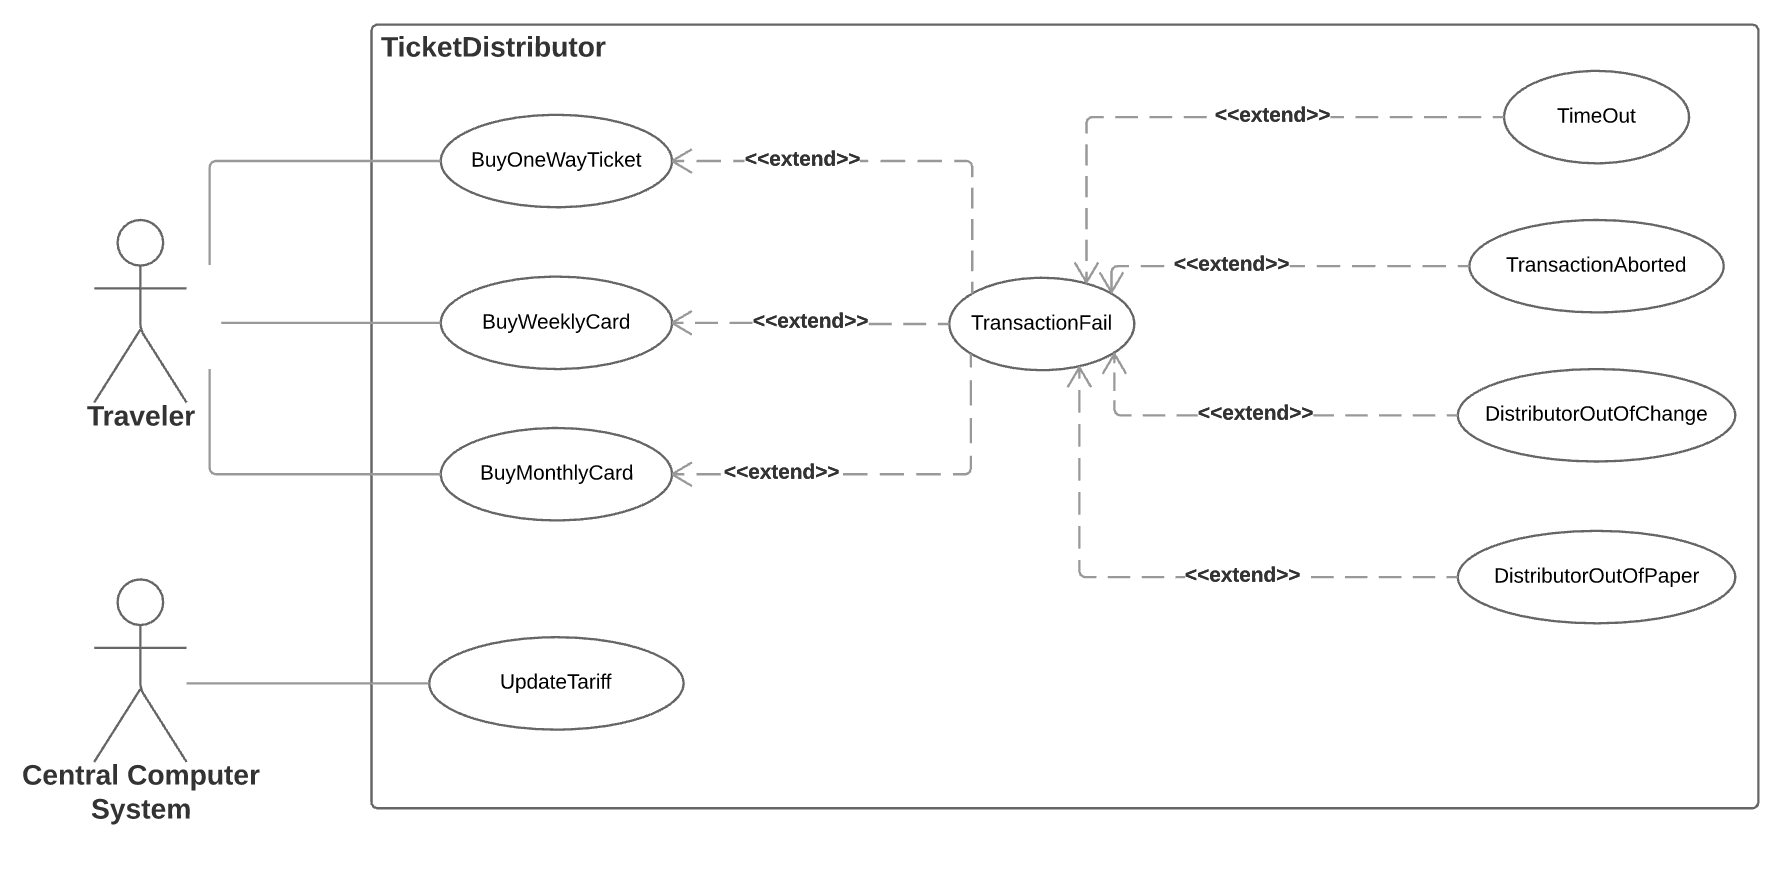
\includegraphics[width=\textwidth]{UseCaseDiagram}
\centering
\end{figure}

\section{Exercise 3}

\subsection{}
Consider the process of ordering a pizza over the phone. Draw an activity diagram representing each step of the process, from the moment you pick up the phone to the point where you start eating the pizza. Do not represent any exceptions. Include activities that others need to perform.\\
\\
\textbf{Answer:} 
\begin{figure}[H]
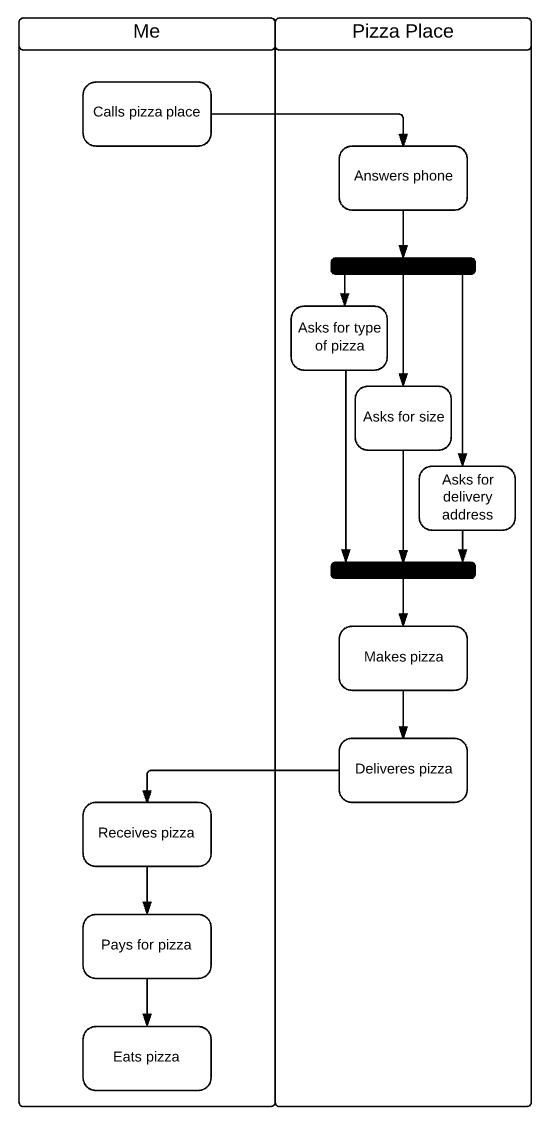
\includegraphics[]{ActivityWOE}
\centering
\end{figure}

\subsection{}
Add exception handling to the activity diagram you developed in the previous exercise. Consider at least three exceptions. You can for instance use the following: delivery person wrote down wrong address, deliver person brings wrong pizza, store out of anchovies.\\
\\
\textbf{Answer:} 
\begin{figure}[H]
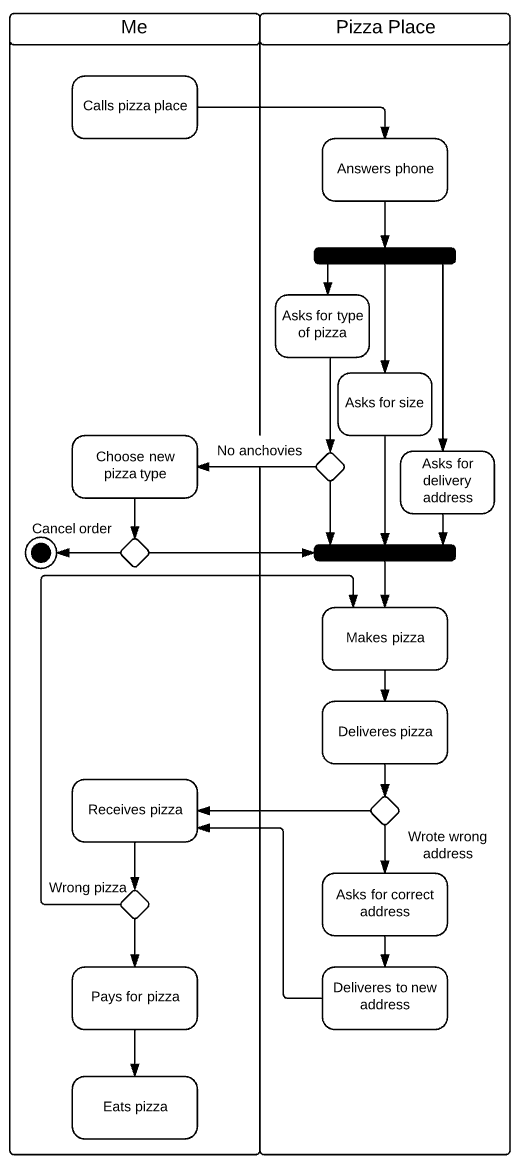
\includegraphics[]{ActivityWE}
\centering
\end{figure}

\section{C\#}
Github link: \url{https://github.itu.dk/marw/BDSA2017.Assignment03}



\end{document}